\chapter{METODOLOGI}
\section{Metode Pencarian Solusi Optimisasi}
  Untuk mencari solusi optimisasi pendeteksian objek kecil YOLOv7 yang terbaik, akan dilakukan penambahan atau perubahan \emph{bag-of-freebies}, \emph{bag-of-specials}, dan arsitektur YOLOv7.
  Setiap modifikasi-modifikasi itu akan diaplikasikan secara independen dan kombinatif.
  Yang dimaksud dengan kombinatif adalah modifikasi-modifikasi akan dikombinasikan menjadi 1 model YOLOv7.

  Setiap kombinasi modifikasi, independen atau tidak, akan diuji kemampuannya mendeteksi objek \emph{airborne}.
  Solusi optimisasi terbaik akan ditentukan berdasarkan metrik $AP_{50}$.
  Subbab \ref{section:modificationcandidates} akan membahas tentang kandidat modifikasi-modifikasi yang dapat dilakukan.

  Tahapan pencarian solusi optimisasi sendiri dapat dibagi menjadi enam tahap.
  Tahap-tahap tersebut adalah Persiapan Dataset, Pembuatan \emph{Auto-trainer}, Pembuatan Konfigurasi Modifikasi, \emph{Training Model}, Analisis, dan Pemilihan Model Terbaik.
  Urutan pengerjaan dari tahap-tahap ini dapat dilihat pada Gambar \ref{fig:metodologi}.
  \begin{figure}[ht]
    \centering
    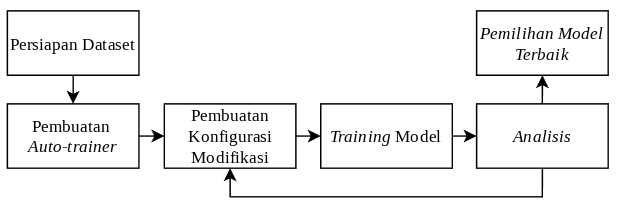
\includegraphics[scale=0.8]{pictures/metodologi.png}
    \caption{Urutan Pengerjaan Penelitian}
    \label{fig:metodologi}
  \end{figure}
  %insert diagram modifikasi here
  %Menyiapkan dataset, Membuat \emph{auto-trainer}, Membuat konfigurasi-konfigurasi modifikasi, Melatih model-model YOLOv7 yang sudah dimodifikasi,
  %Menganalisis performa hasil modifikasi YOLOv7, dan Pemilihan model modifikasi YOLOv7 dengan skor mAP terbaik.

  Pada tahap persiapan dataset, akan dilakukan pengunduhan dataset dari \textcite{aot_dataset}.
  Gambar-gambar pada dataset ini kemudian akan di-\emph{sampling} dan didistribusikan menjadi dataset \emph{training}, validasi, dan pengujian.
  Pada pendistribusian dataset ini juga akan dilakukan \emph{balancing} antar kelas dan dataset positif negatif.
  \emph{Balancing} dilakukan agar tidak ada kelas yang mendominasi pada dataset.

  Selanjutnya, di tahap pembuatan \emph{auto-trainer}, akan dilakukan pembuatan program yang dapat dengan otomatis membangun dan melatih \emph{neural network} modifikasi YOLOv7.
  Pembuatan \emph{auto-trainer} ini dilakukan agar proses-proses pengerjaan tahapan-tahapan selanjutnya menjadi dapat dilakukan dengan lebih mudah.

  Setelah itu, akan dilakukan pembuatan konfigurasi-konfigurasi modifikasi.
  Konfigurasi modifikasi YOLOv7 akan dibuat agar dapat diinputkan pada \emph{auto-trainer}.
  Konfigurasi modifikasi akan berisi kombinasi modifikasi-modifikasi yang ada pada subbab \ref{section:modificationcandidates}.

  Tahapan selanjutnya adalah \emph{Training} model.
  Pada tahap ini, konfigurasi-konfigurasi modifikasi pada tahapan sebelumnya akan dibangun dan kemudian dilatih.
  Hasil dari tahap ini adalah \emph{weights neural network} modifikasi YOLOv7, histori pelatihannya, dan metrik-metriknya pada dataset uji.

  Pada tahap analisis, hasil dari tahap sebelumnya akan dianalisis untuk mencari tahu performa model-model hasil modifikasi.
  Analisis juga dilakukan untuk menemukan \emph{gap} kandidat modifikasi lain yang masih bisa dieksplorasi untuk meningkatkan kemampuan pendeteksian objek kecil YOLOv7.
  Ketika suatu kandidat modifikasi seperti itu ditemukan, maka akan dilakukan kembali pembuatan konfigurasi modifikasi untuk menguji kandidat modifikasi tersebut.

  Tahapan terakhir adalah pemilihan model terbaik.
  Pada tahapan ini akan dipilih model yang memiliki performa terbaik dari antara model-model hasil modifikasi lainnya.
  Pemilihan model akan dilakukan dengan berdasarkan pada skor mAP tertinggi.
  Untuk mempertahankan solusi optimisasi yang dapat melakukan deteksi secara \emph{real time}, model yang akan dipilih hanyalah model yang dapat melakukan deteksi dengan kecepatan minimum 10 FPS pada \emph{onboard computing device} seperti Jetson TX2 atau \emph{compute device} lainnya.


\section{Kandidat Modifikasi}
\label{section:modificationcandidates}
  \subsection{Rekalkulasi \emph{Anchor On-Training}}
    Yang dimaksud dengan rekalkulasi \emph{anchor on-training}  adalah ketika ukuran-ukuran \emph{anchor box} direkalkulasi pada saat training.
    Berbeda dengan \emph{clustering pre-training} seperti pada YOLOv2 \parencite{yolov2}, ukuran-ukuran \emph{anchor} akan di-\emph{learning} bersama dengan pendeteksi objeknya.
    Untuk melakukan hal ini, digunakan algoritma optimisasi \emph{anchor box} yang mirip dengan algoritma \textcite{anchoropt}.
    Pada bagian \emph{head}, akan ditempelkan suatu layer yang akan mengoutputkan faktor \emph{rescaling} dari tiap \emph{anchor box}.
    Bagian tersebut akan di-\emph{training} bersama dengan YOLOv7 \emph{anchor box} akan teroptimisasi tidak hanya pada dataset, namun pada keseluruhan \emph{neural network} juga.
  \subsection{Augmentasi Mosaik}
    Berbeda dengan versi YOLO sebelumnya \parencites{yolov4}{yolov5}, YOLOv7 tidak menggunakan augmentasi mosaik.
    Padahal, dapat dilihat dari YOLOv4, augmentasi mosaik dapat meningkatkan akurasi deteksi.
    Oleh karena itu, akan dilakukan percobaan penambahan augmentasi mosaik pada YOLOv7 untuk melihat apakah augmentasi mosaik ini akan meningkatkan akurasinya atau tidak.
  \subsection{Modifikasi Neck}
    \begin{figure}[ht]
      \centering
      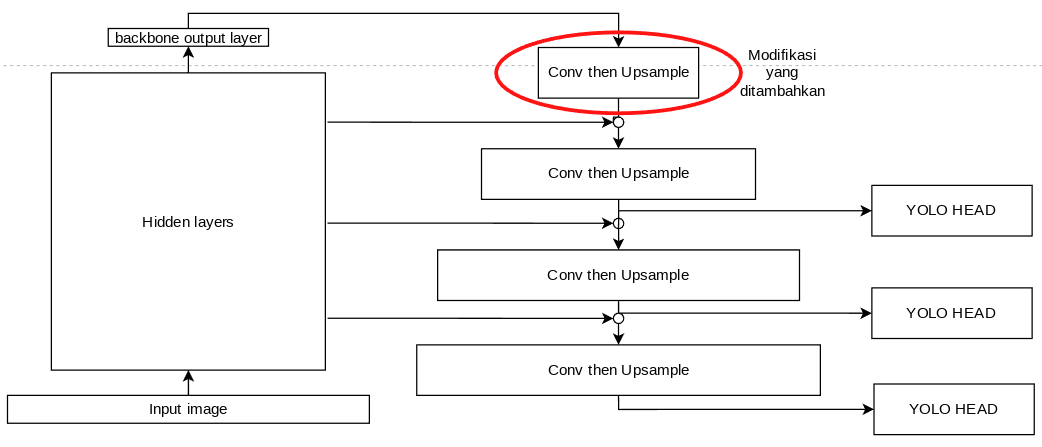
\includegraphics[scale=0.5]{pictures/add-more-upsampling.png}
      \caption{Menambah \emph{upsampling} pada \emph{neck}}
      \label{fig:neckaddupsampling}
    \end{figure}
    \begin{figure}[ht]
      \centering
      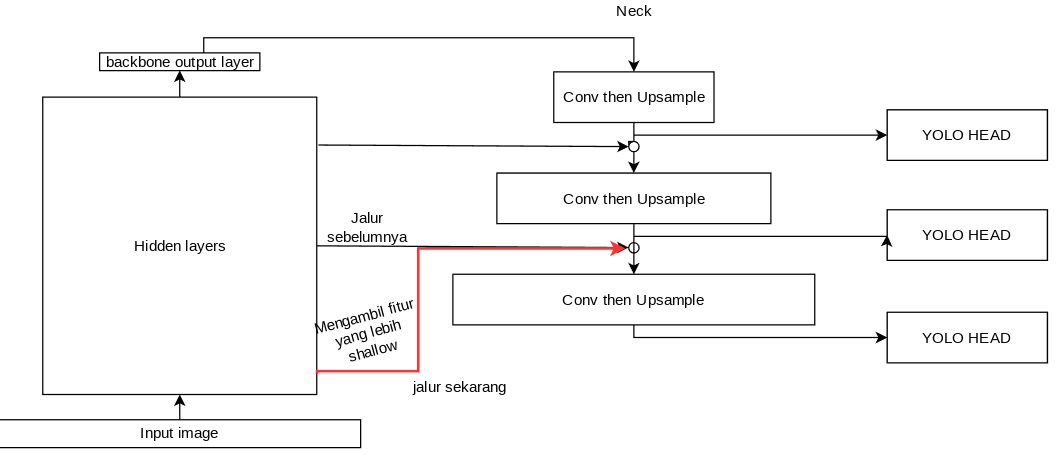
\includegraphics[scale=0.5]{pictures/neck-move-back.png}
      \caption{Menggunakan \emph{feature map} dari layer yang lebih di belakang}
      \label{fig:neckmoveback}
    \end{figure}
    Seperti pada penelitian-penelitian terkait di subbab \ref{section:relatedwork}, modifikasi \emph{neck} dapat dilakukan untuk meningkatkan akurasi pendeteksian objek kecil.
    Modifikasi \emph{neck} dapat dilakukan dengan menambahkan layer upsampling seperti pada Gambar \ref{fig:neckaddupsampling} atau dengan memindahkan sumber feature map untuk dari beberapa layer neck lebih jauh ke belakang seperti pada Gambar \ref{fig:neckmoveback}.
    Penambahan layer upsampling dapat membuat neural network untuk mendapatkan feature-map yang lebih detail sehingga dapat melakukan pendeteksian objek kecil dengan lebih baik.
    Pemindahan sumber feature map ke belakang dapat dilakukan untuk mengantisipasi fitur objek kecil yang dapat hilang ketika layer neural network semakin dalam.
    Dengan memindahkannya lebih ke belakang, YOLOv7 akan melakukan deteksi pada layer dengan abstraksi yang lebih rendah (sedikit informasi yang hilang).
  \subsection{Penambahan YOLO Head}
    \begin{figure}[ht]
      \centering
      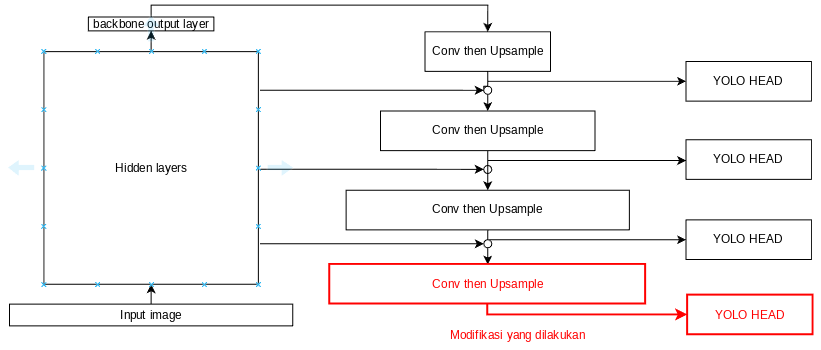
\includegraphics[scale=0.65]{pictures/addmorehead.png}
      \caption{Penambahan \emph{Layer} Head pada YOLO}
      \label{fig:addmorehead}
    \end{figure}
    Penambahan YOLO head dapat membuat YOLOv7 melakukan deteksi pada skala yang lebih tinggi.
    Hal ini akan berpengaruh pada kemampuan pendeteksian objek kecil.
    Dengan melakukan pendeteksian pada skala yang lebih beragam, YOLOv7 dapat mendeteksi objek yang besar maupun kecil.
    Perhatikan bahwa penambahan YOLO Head akan diikuti dengan penambahan \emph{layer upsampling} pada \emph{neck} seperti di Gambar \ref{fig:addmorehead}.
    
\section{Dataset}
  \subsection{Sumber Dataset}
    Dataset untuk objek-objek \emph{airborne} didapatkan dari \textcite{aot_dataset} dan dihost pada suatu server AWS S3 Bucket.
    Dataset ini berisi video-video monokromatik penerbangan UAV.
    Terdapat 4 kelas pada dataset ini yaitu pesawat, helikopter, burung, dan \emph{other}.
    Distribusi dataset training dan uji dapat dilihat pada tabel \ref{tbl:datasettraintest} sedangkan distribusi kelas dari dataset dapat dilihat pada Tabel \ref{tbl:datasetclasses}.
    \begin{table}[h]
      \centering
      \captionof{table}{Distribusi Dataset Training dan Test}
      \label{tbl:datasettraintest}
      \begin{tabular}{|c|c|c|c|c|}
        \hline
        Pembagian & Ukuran (TB) & Sekuen penerbangan & Jumlah Gambar & Jumlah Label\\
        Dataset &  & UAV &  & \\
        \hline
        Training & 11,3 & 4154 & 4975765 & 2891891\\
        \hline
        Validation + Test &2.1 &789 & 943852 & 496075\\
        \hline
        Total &13,4 &4943 & 5919617 & 3387966\\
        \hline
      \end{tabular}
    \end{table}

    \begin{table}[h]
      \centering
      \captionof{table}{Distribusi Kelas Dataset}
      \label{tbl:datasetclasses}
      \begin{tabular}{|c|c|c|c|c|c|}
        \hline
        Pembagian & Total Objek & Pesawat & Helikopter & Burung & \emph{Other}\\
        \hline
        Training & 2,89 juta & 0,79 juta& 1,22 juta& 0,33 juta& 0,54 juta\\
        \hline
        Validation + Test &0,50 juta &0,13 juta & 0,17 juta&0,06 juta&0,14 juta\\
        \hline
        Total &3,39 juta &0,92 juta & 1,39 juta&0,39 juta&0,69 juta\\
        \hline
      \end{tabular}
    \end{table}
  
  \subsection{Sampling Dataset}
    Karena jumlah dataset pada \textcite{aot_dataset} berukuran sangat besar, hanya sebagian dari dataset tersebut akan digunakan untuk \emph{training} dan \emph{test}.
    Akan diambil total 60000 gambar dari dataset dengan pembagian sesuai dengan Tabel \ref{tbl:datasetsamplingdist}
    \begin{table}[h]
      \centering
      \captionof{table}{Distribusi Sampling Dataset}
      \label{tbl:datasetsamplingdist}
      \begin{tabular}{|c|c|c|c|c|c|c|}
        \hline
        Pembagian &Total & \multicolumn{4}{c}{Presentase}&\\
                           \cline{2-7}
                  &Gambar& Pesawat & Helikopter & Burung & \emph{Other} & Negatif\\
        \hline
        Training  &54000 &23,75\%  &23,75\%     &23,75\% &23,75\%       &5\%\\
        \hline                                              
        Validation&3000  &20\%     &20\%        &20\%    &20\%          &20\%\\
        \hline                                                           
        Test      &3000  &20\%     &20\%        &20\%    &20\%          &20\%\\
        \hline
      \end{tabular}
    \end{table}

    %Untuk membagi dataset agar terdistribusi seperti pada Tabel \ref{tbl:datasetsamplingdist}, akan digunakan algoritma seperti berikut:
    %\begin{algorithmic}
    %  \State $L_0 \gets$ List index gambar-gambar yang memiliki objek kelas pesawat
    %  \State $L_1 \gets$ List index gambar-gambar yang memiliki objek kelas helikopter
    %  \State $L_2 \gets$ List index gambar-gambar yang memiliki objek kelas burung 
    %  \State $L_3 \gets$ List index gambar-gambar yang memiliki objek kelas \emph{Other}
    %  \State $L_4 \gets$ List index gambar-gambar yang memiliki objek kelas negatif
    %  \For{$i \gets 0$ to $4$}
    %    \State $L_i \gets shuffle(L_i)$
    %  
    %  

    %\end{algorithmic}




\section{Skema Training Model}
  Untuk melatih berbagai modifikasi YOLOv7, akan dibuat suatu \emph{auto-trainer}.
  \emph{Auto-trainer} ini akan menerima suatu \emph{file} konfigurasi modifikasi YOLOv7, dan dengan otomatis membangun arsitektur YOLOv7 yang termodifikasi dan melatihnya.
  Setelah mendapatkan model modifikasi YOLOv7 yang sudah dilatih, \emph{auto-trainer} akan menguji model tersebut dengan dataset uji.
  Metrik-metrik pengujian, grafik histori \emph{training loss vs validation loss}, dan \emph{weights} dari model kemudian akan dikirim ke user.
  Dengan membuat \emph{auto-trainer} ini, proses pelatihan model dan pelaporan hasil menjadi terotomasi sehingga akan mempermudah proses penelitian.

\section{Timeline Pelaksanaan Penelitian}
  \newcommand{\w}{}
  \newcommand{\G}{\cellcolor{gray}}
  \begin{table}[h!]
    \captionof{table}{Tabel timeline}
    \label{tbl:timeline}
    \begin{tabular}{|p{3.5cm}|c|c|c|c|c|c|c|c|c|c|c|c|c|c|c|c|}
  
      \hline
      \multirow{2}{*}{Kegiatan} & \multicolumn{16}{|c|}{Minggu} \\
      \cline{2-17} &
      1 & 2 & 3 & 4 & 5 & 6 & 7 & 8 & 9 & 10 & 11 & 12 & 13 & 14 & 15 & 16 \\
      \hline
  
      % Gunakan \G untuk mengisi sel dan \w untuk mengosongkan sel
      Persiapan Dataset &
      \G & \w & \w & \w & \w & \w & \w & \w & \w & \w & \w & \w & \w & \w & \w & \w \\
      \hline
  
      Pemb. \emph{Auto-trainer} &
      \w & \G & \w & \w & \w & \w & \w & \w & \w & \w & \w & \w & \w & \w & \w & \w \\
      \hline
  
      Pemb. Konfigurasi&
      \w & \w & \G & \G & \G & \G & \G & \G & \G & \G & \G & \G & \w & \w & \w & \w \\
      Modifikasi &
      \w & \w & \G & \G & \G & \G & \G & \G & \G & \G & \G & \G & \w & \w & \w & \w \\
      \hline
  
      Training Model &
      \w & \w & \G & \G & \G & \G & \G & \G & \G & \G & \G & \G & \w & \w & \w & \w \\
      \hline

      Analisis &
      \w & \w & \G & \G & \G & \G & \G & \G & \G & \G & \G & \G & \G & \w & \w & \w \\
      \hline

      Pemb. Laporan &
      \w & \w & \w & \w & \w & \w & \w & \w & \w & \w & \w & \w & \G & \G & \G & \G \\
      \hline
  
    \end{tabular}
  \end{table}
